\section{Applied Design Patterns}
\label{sec:applied-design-patterns}
\begingroup
\sloppy

The project uses design patterns at several different scales.  Some patterns
control the lifetime and navigation of the application, some provide extension
points for gameplay objects, and others isolate the creation of families of
entities.  Table~\ref{tab:pattern-summary} gives the principal mapping from the
pattern vocabulary to the concrete implementation.

\begin{table}[htbp]
    \centering
    \small
    \renewcommand{\arraystretch}{1.2}
    \begin{tabular}{|p{0.16\textwidth}|p{0.34\textwidth}|p{0.39\textwidth}|}
        \hline
        \textbf{Pattern} & \textbf{Principal participants} & \textbf{Purpose in the game} \\
        \hline
        Singleton & \texttt{Game} & Provides one process-wide window, state stack, audio service, and selected character/level configuration. \\
        \hline
        Factory & \texttt{HeroFactory}, \texttt{EnemyFactory}, \texttt{BlockFactory}, \texttt{ItemFactory}, \texttt{ProjectileFactory}, \texttt{EnemyStateFactory} & Converts compact types or saved/map strings into polymorphic runtime objects. \\
        \hline
        State & Application \texttt{State}; \texttt{HeroState}; \texttt{EnemyState} & Represents screens, hero movement modes, and enemy/boss AI modes without large central conditionals. \\
        \hline
        Strategy & \texttt{HeroForm} with \texttt{SmallForm}, \texttt{GiantForm}, and \texttt{FireForm} & Changes size, texture, input capabilities, special attack policy, and damage response at run time. \\
        \hline
        Observer & Sound/projectile callbacks and HUD notifications & Propagates gameplay events to the world, sound service, and display without giving entities ownership of those receivers. \\
        \hline
        Prototype & \texttt{Item::clone}, especially \texttt{PowerUpPrototype} & Lets a block retain one item description and create context-sensitive rewards when hit. \\
        \hline
        Facade & \texttt{LevelRuntime} & Presents one update/render interface over world ownership, construction, physics, interactions, regions, pipes, and goals. \\
        \hline
        Factory Method & \texttt{Hero::createSpecialProjectile} & Allows the invariant special-ability workflow to create a hero-specific projectile. \\
        \hline
        Object Pool & \texttt{SoundManager::m\_sfxPool} & Reuses a bounded number of SFML sound channels for overlapping effects. \\
        \hline
    \end{tabular}
    \caption{Design patterns identified in the current implementation.}
    \label{tab:pattern-summary}
\end{table}

\subsection{Singleton Pattern}
\label{subsec:singleton-pattern}

\subsubsection{Intent and participants}

The Singleton pattern ensures that a class has one instance and supplies a
global access point to it.  The project applies the pattern to \texttt{Game}.
Its constructor is private, its copy constructor and assignment operator are
deleted, and \texttt{Game::getInstance()} returns a function-local static
instance.  This is the ``Meyers Singleton'' form: construction occurs on first
use, and C++ guarantees thread-safe initialization of the local static object.

\begin{figure}[htbp]
\centering
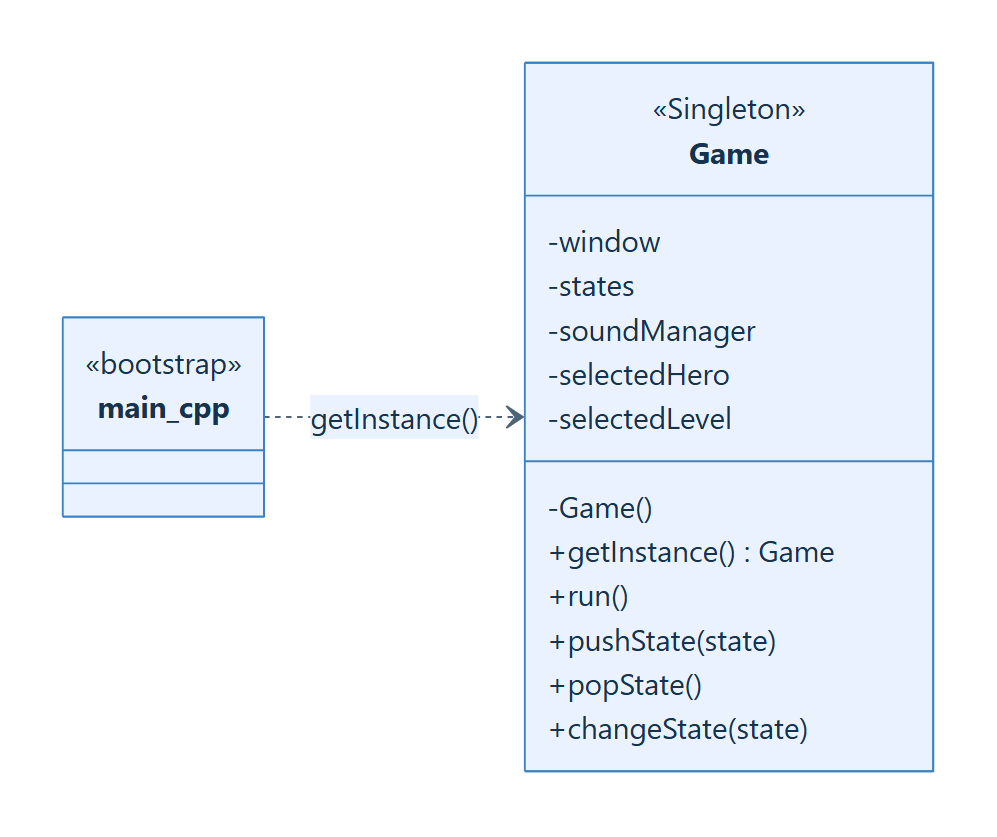
\includegraphics[width=0.56\textwidth,height=0.56\textheight,keepaspectratio]{img/diagrams/pattern-singleton.png}
\caption{The single \texttt{Game} object owns process-wide application state.}
\end{figure}

The bootstrap in \texttt{src/main.cpp} obtains the instance twice: first to
queue a \texttt{MainMenuState}, and then to start \texttt{run()}.  Screen
objects use the same access point to request state transitions, obtain the
\texttt{SoundManager}, and read or update the selected hero, selected level,
and volume settings.

\subsubsection{Why it fits}

SFML should have one authoritative render window and one main loop.  Likewise,
the state stack and deferred transition request must agree on which screen is
active.  Centralizing these resources prevents accidental creation of a second
window, independent audio service, or competing navigation stack.  The
function-local static also avoids the static-initialization-order problem that
would arise from a namespace-scope \texttt{Game} object.

The cost is global coupling: states call \texttt{Game::getInstance()} directly,
which makes isolated unit tests harder and makes dependencies less visible in
constructors.  This is acceptable for the current small application shell, but
future testing could introduce narrow interfaces such as a state navigator or
audio service and inject those interfaces while retaining a single production
\texttt{Game} instance.

\subsection{Factory Patterns}
\label{subsec:factory-patterns}

\subsubsection{Simple factories for entity families}

The project uses several centralized creation functions.  Each returns a
\texttt{std::unique\_ptr} to an abstract or base type, hiding concrete
constructors from the caller:

\begin{itemize}
    \item \texttt{HeroFactory::createHero} maps \texttt{HeroType} to
    \texttt{Mario}, \texttt{Luigi}, or \texttt{Flash}, while forwarding the
    projectile-spawn callback.
    \item \texttt{EnemyFactory::createEnemy} maps \texttt{EnemyType} to
    \texttt{Goomba}, \texttt{Koopa}, \texttt{Witch}, or \texttt{ThorKing}.
    Its string overload supports map and persistence data.
    \item \texttt{BlockFactory::createBlock} builds \texttt{BrickBlock},
    \texttt{QuestionBlock}, or \texttt{InvisibleBlock}, attaches a hidden item
    prototype, and supplies the shared \texttt{BlockThemePalette} where needed.
    \item \texttt{ItemFactory::createItem} supports both the enum-based level
    builder and the string-based save loader.
    \item \texttt{ProjectileFactory::createProjectile} reconstructs hero and
    enemy projectiles from saved type names, velocities, and factions.
    \item \texttt{EnemyStateFactory::createStateFromString} reconstructs
    ordinary enemy AI states such as \texttt{Patrol}, \texttt{Squished},
    \texttt{Shell}, \texttt{SpinningShell}, \texttt{FlippingDeath}, and
    \texttt{Throw}.
\end{itemize}

\begin{figure}[htbp]
\centering
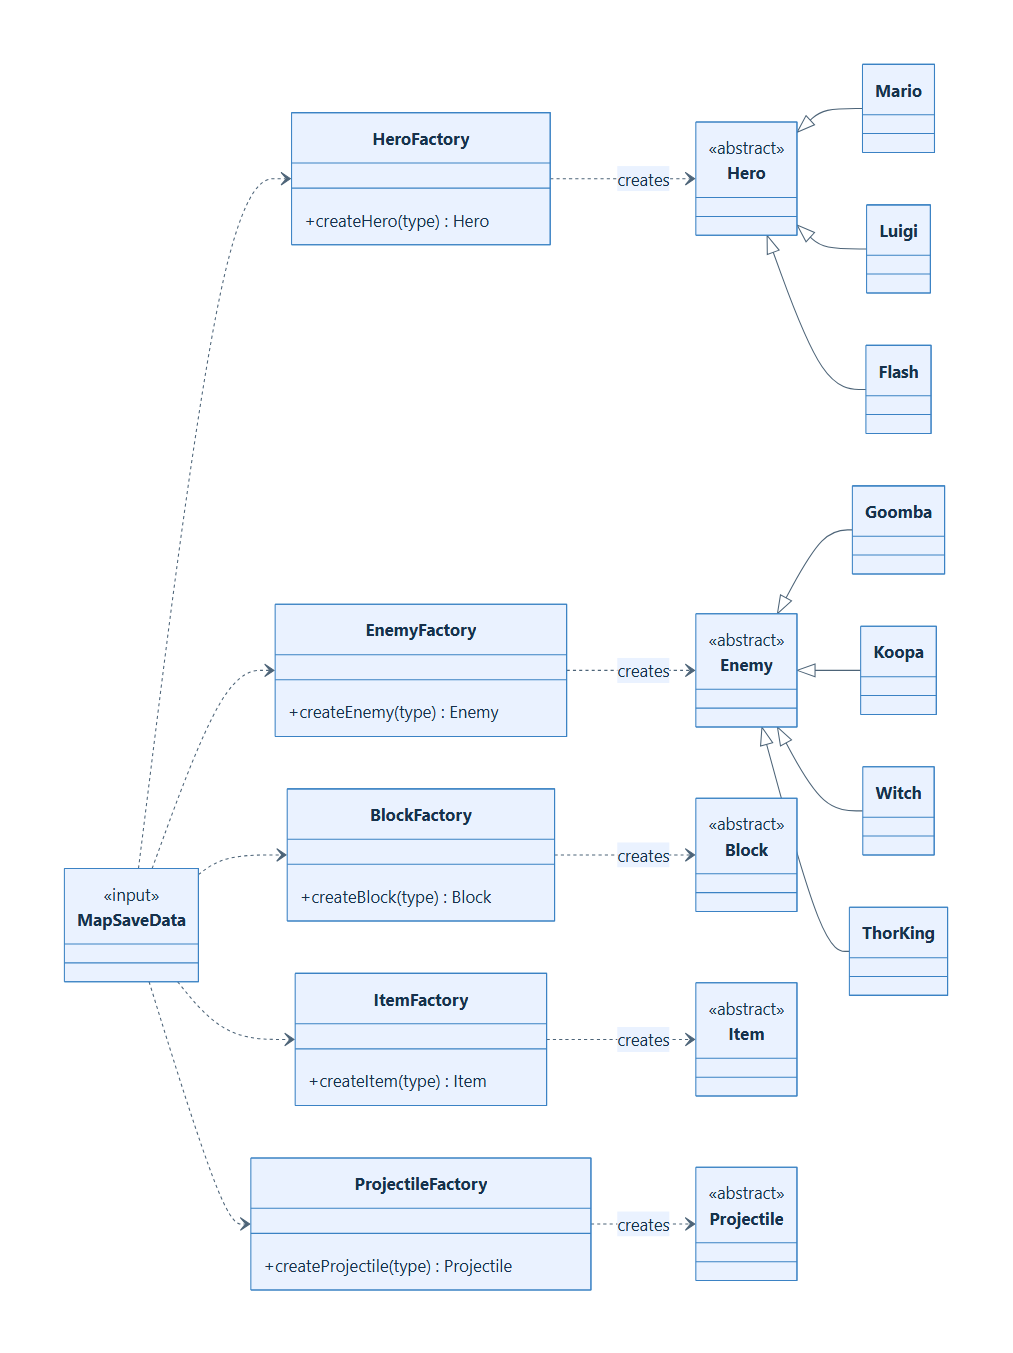
\includegraphics[width=0.68\textwidth,height=0.70\textheight,keepaspectratio]{img/diagrams/pattern-factories.png}
\caption{Factories translate data-oriented identifiers into owned polymorphic objects.}
\end{figure}

This design is especially important at the data boundary.  \texttt{LevelBuilder}
does not need sprite initialization details for every entity, and
\texttt{SaveManager} does not depend on every concrete constructor.  Adding a
new product normally requires a new concrete class, one factory mapping, and
the relevant builder or serialization mapping rather than changes throughout
the game loop.

\subsubsection{Polymorphic factory interface}

\texttt{BaseEnemyFactory} with \texttt{ConcreteGoombaFactory} and
\texttt{ConcreteKoopaFactory} is the project's explicit polymorphic factory
hierarchy.  A client can hold a \texttt{BaseEnemyFactory} reference and call
\texttt{create()} without knowing the product type.  The current runtime mainly
uses the static \texttt{EnemyFactory}; therefore the concrete factory hierarchy
is a valid extension point but is not the primary construction route.

\subsubsection{Factory Method for hero attacks}

The hero special attack is a smaller Factory Method example.  The public
\texttt{Hero::specialAbility()} method owns the stable algorithm: verify that a
spawn callback exists, ask for a projectile, and transfer ownership to the
world.  The protected pure virtual
\texttt{createSpecialProjectile()} is overridden by each hero:

\begin{itemize}
    \item \texttt{Mario} creates a bouncing \texttt{MarioFireball};
    \item \texttt{Luigi} creates an arcing \texttt{LuigiWaterBomb};
    \item \texttt{Flash} creates a fast \texttt{FlashThunder} strike.
\end{itemize}

Thus the base class fixes when and how an attack is published, while subclasses
decide what concrete product is created.

\subsection{State Pattern}
\label{subsec:state-pattern}

The project applies State three times.  These applications have the same
intent---delegating behavior to a replaceable object---but operate at different
levels and should not be confused with one another.

\subsubsection{Application and screen states}

\texttt{State} defines the common \texttt{processEvents}, \texttt{update}, and
\texttt{render} operations.  \texttt{Game} owns a stack of
\texttt{std::unique\_ptr<State>} and forwards each event/update to the top
state.  Rendering may include lower states when the top state returns
\texttt{true} from \texttt{rendersBelow()}, which is used by modal overlays such
as pause, continue prompt, and victory.

The concrete states are \texttt{MainMenuState}, \texttt{ContinuePromptState},
\texttt{CharacterSelectState}, \texttt{LevelSelectState}, \texttt{GuideState},
\texttt{SettingsState}, \texttt{TransitionState}, \texttt{PlayingState},
\texttt{PausedState}, \texttt{VictoryState}, and \texttt{GameOverState}.
Transitions are requested with \texttt{pushState}, \texttt{popState},
\texttt{changeState}, or \texttt{clearStatesAndChange}.  \texttt{Game} defers
the request until it is outside the outgoing state's callback, preventing an
object from being destroyed while one of its methods is still executing.

\begin{figure}[htbp]
\centering
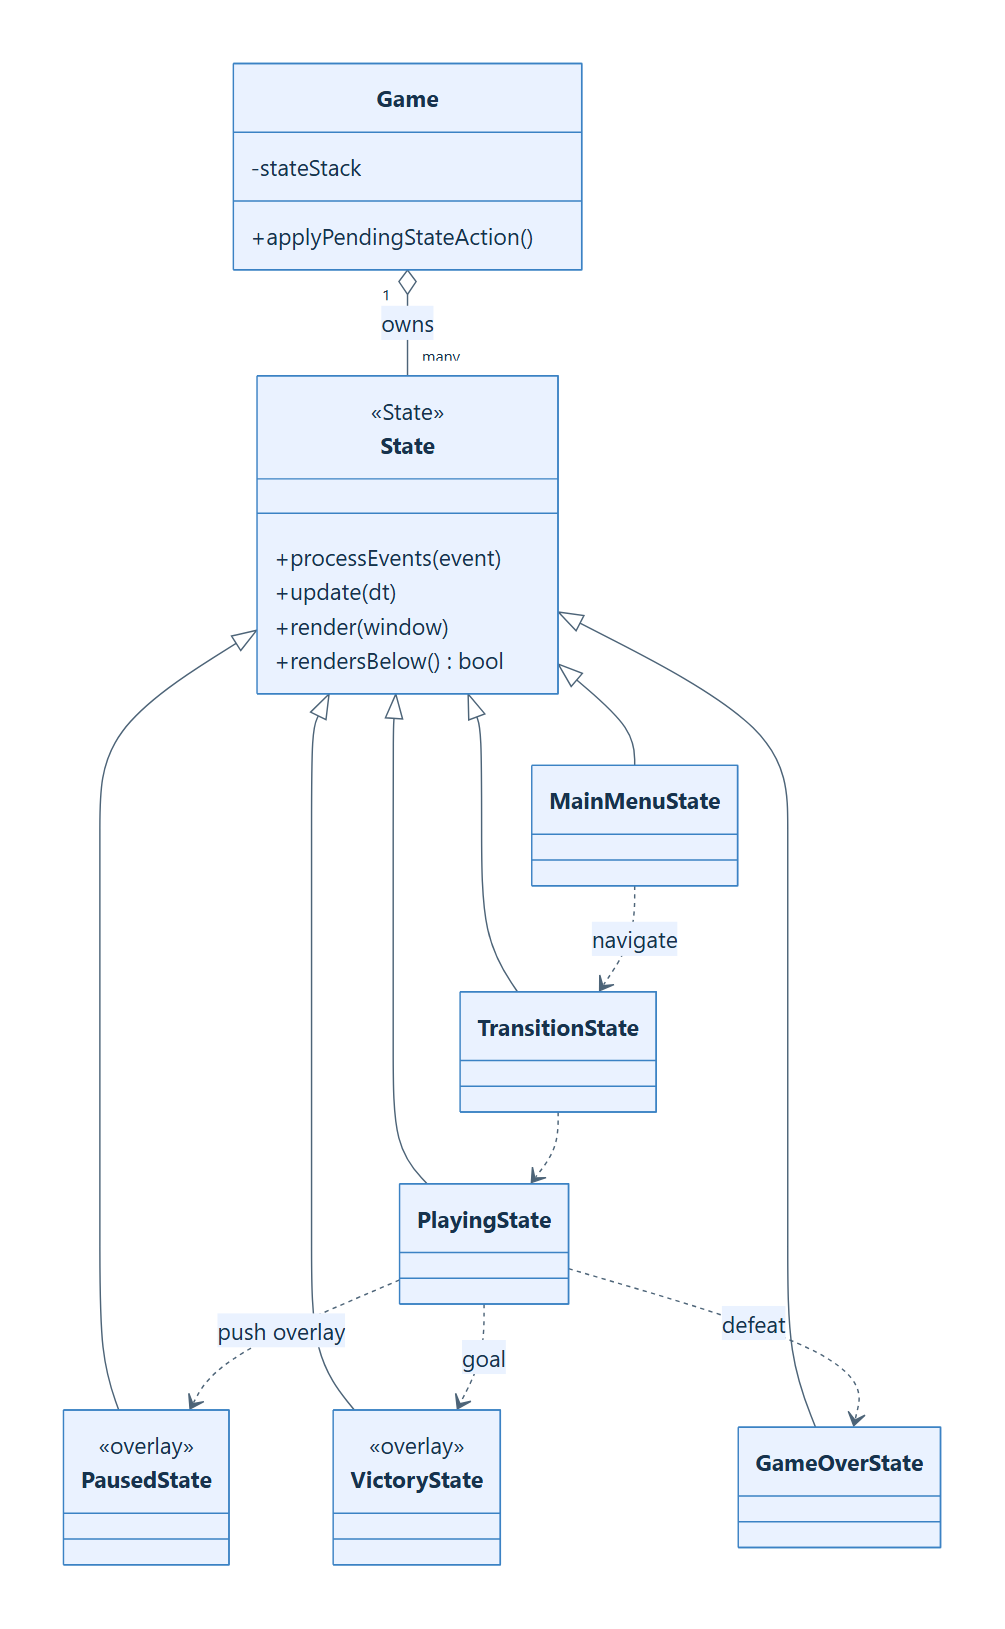
\includegraphics[width=0.68\textwidth,height=0.70\textheight,keepaspectratio]{img/diagrams/pattern-state.png}
\caption{Application State pattern and the state stack.}
\end{figure}

\subsubsection{Hero movement states}

\texttt{Hero} owns exactly one \texttt{HeroState}.  The interface supplies
\texttt{enter}, \texttt{exit}, \texttt{update}, and \texttt{getState}.  The
concrete states are \texttt{IdleState}, \texttt{RunState}, \texttt{JumpState},
\texttt{SlideState}, \texttt{SitState}, \texttt{GrowState},
\texttt{ShrinkState}, \texttt{DeadState}, and \texttt{CheerState}.  State
objects interpret input, set velocity, alter the hitbox when necessary, select
animations through their names, and initiate transitions by calling
\texttt{Hero::setState}.

For example, an idle hero enters \texttt{RunState} when horizontal input is
held, \texttt{JumpState} when jumping, and \texttt{SitState} when a powered
form crouches.  Reversing direction while moving can enter
\texttt{SlideState}.  Transformation states temporarily lock motion before
installing a new form, while \texttt{DeadState} and \texttt{CheerState} suppress
normal control for defeat and victory respectively.  \texttt{JumpState}'s
\texttt{AirEntry} value distinguishes a deliberate jump from walking off a
ledge.

\subsubsection{Enemy and boss AI states}

\texttt{Enemy} similarly owns an \texttt{EnemyState}.  Its
\texttt{changeState} method calls \texttt{onExit} on the old object and
\texttt{onEnter} on the new object.  General states implement patrolling,
squishing, a stationary shell, a spinning shell, and flipping death.
\texttt{Witch} adds \texttt{ThrowState}.  \texttt{ThorKing} extends the same
interface with \texttt{TKPatrolState}, \texttt{TKCrouchState},
\texttt{TKRollingState}, \texttt{TKStunnedState},
\texttt{TKFireAttackState}, and \texttt{TKRoarState}.  These objects express
multi-phase boss behavior while the \texttt{ThorKing} entity retains shared HP,
phase counters, movement data, projectile callback, and sound callback.

The State design localizes transition rules and makes save/load possible:
ordinary enemy state names are mapped back to state objects by
\texttt{EnemyStateFactory}.  The present persistence code restores Thor King's
counters and resumes it in a patrol state, so not every transient boss timer is
serialized.

\subsection{Strategy Pattern}
\label{subsec:strategy-pattern}

\texttt{HeroForm} is a Strategy family installed inside \texttt{Hero} alongside
the independent movement-state object.  Its operations---\texttt{enter},
\texttt{update}, \texttt{getForm}, and \texttt{takedamage}---represent the
parts of hero behavior that vary with power level rather than movement mode.

\begin{figure}[htbp]
\centering
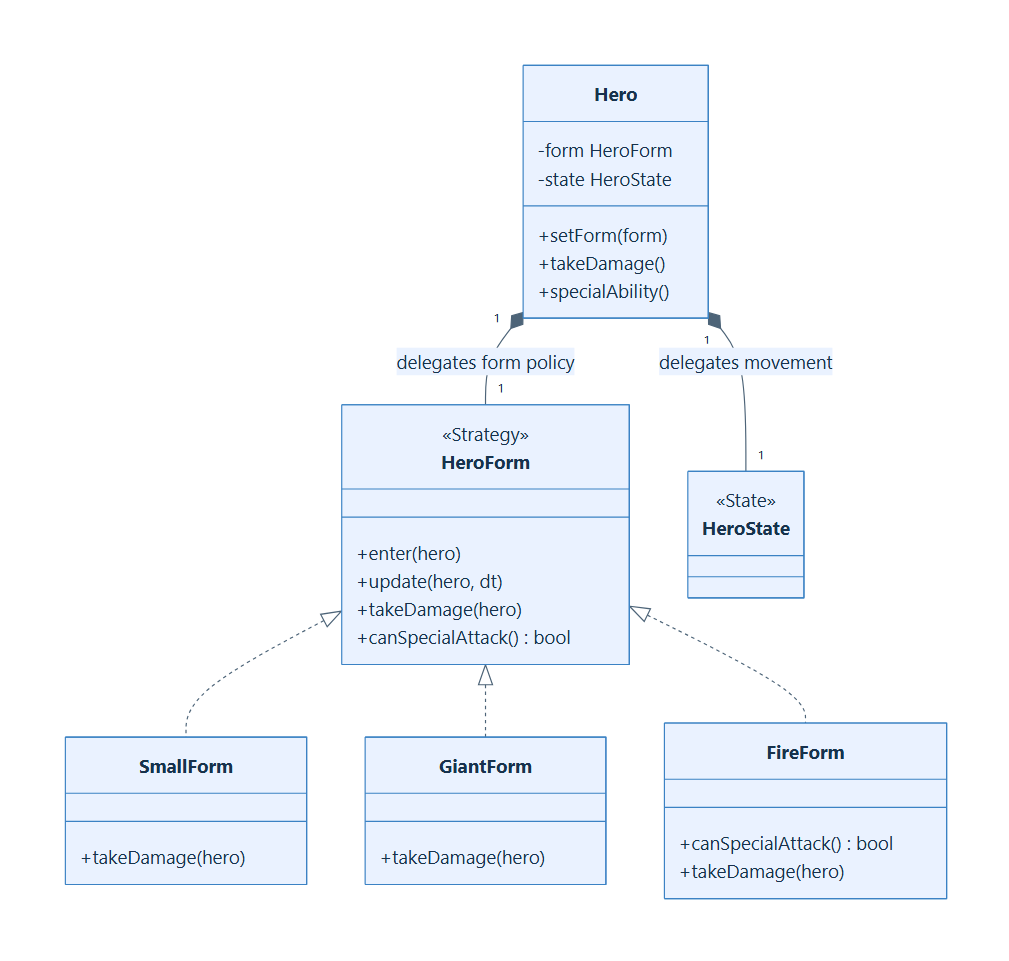
\includegraphics[width=0.82\textwidth,height=0.58\textheight,keepaspectratio]{img/diagrams/pattern-strategy.png}
\caption{Hero form is a run-time strategy independent of movement state.}
\end{figure}

\texttt{SmallForm} selects the base texture and a $32\times32$ hitbox and dies
on damage.  \texttt{GiantForm} uses a $32\times64$ standing hitbox, permits
crouching, and changes damage into a shrink transition.  \texttt{FireForm}
loads each hero's special texture, applies a per-hero cooldown, invokes the
Factory Method for the special projectile, and downgrades through Giant form
when hit.  For Mario this special strategy is Fire Mario; for Luigi it is the
Kitsune form and water bomb; for Flash it is Thunder Flash and a thunder strike.

This two-axis design prevents a combinatorial class explosion.  The project
does not require classes such as \texttt{RunningFireMario},
\texttt{JumpingGiantLuigi}, or \texttt{SittingThunderFlash}; an animation key is
instead composed from the current form and state names.  Adding a movement
state is mostly independent of adding a power form.

The enemy classes also use small statically composed policy helpers:
\texttt{GoombaPhysics}/\texttt{GoombaAnimator},
\texttt{KoopaPhysics}/\texttt{KoopaAnimator},
\texttt{WitchPhysics}/\texttt{WitchAnimator}, and
\texttt{ThorKingPhysics}/\texttt{ThorKingAnimator}.  They have no shared
strategy interface and are not swapped at run time, so they are best described
as strategy-like separation of physics and presentation rather than a complete
GoF Strategy implementation.

\subsection{Observer Pattern}
\label{subsec:observer-pattern}

The implementation uses a lightweight callback form of Observer.  It avoids
giving gameplay entities pointers to the complete scene and avoids a universal
event bus.  The significant notification channels are:

\begin{itemize}
    \item \texttt{ProjectileSpawnCallback}: \texttt{Hero} publishes a newly
    created projectile; \texttt{GameWorld::addProjectile} is the receiver.
    The same ownership-transfer idea is used by \texttt{Witch} and
    \texttt{ThorKing} for enemy projectiles.
    \item \texttt{Hero::playSFXCallback}: forms and blocks may request effects
    through the hero; \texttt{GameWorld::setHero} connects the callback to the
    non-owning \texttt{SoundManager} service.
    \item \texttt{ThorKing::m\_soundCallback}: the boss publishes
    \texttt{BossSoundEvent::Attack} and \texttt{BossSoundEvent::Defeated}; the
    level builder connects these notifications to the appropriate effects.
    \item HUD notifications: \texttt{PlayingState} observes score deltas, hero
    coin count, lives, time, and the selected world, then invokes
    \texttt{HUDManager}'s update methods.  This is explicit observation rather
    than subscription through an abstract observer interface.
\end{itemize}

\begin{figure}[htbp]
\centering
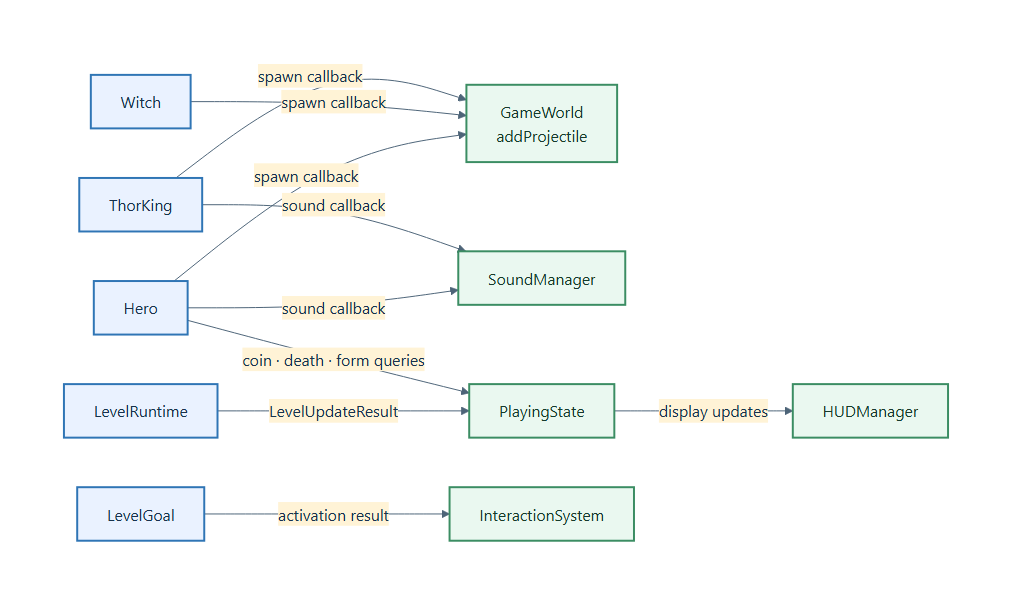
\includegraphics[width=0.94\textwidth,height=0.50\textheight,keepaspectratio]{img/diagrams/pattern-observer.png}
\caption{Callback and explicit-notification form of Observer.}
\end{figure}

The approach keeps ownership clear: a callback transfers a
\texttt{unique\_ptr} when spawning, whereas the audio pointer is non-owning and
outlives the level because it belongs to \texttt{Game}.  Its limitation is that
subscriptions are hand-wired and the HUD is partly polled, so adding many new
event consumers would justify a typed event dispatcher or formal
\texttt{Subject}/\texttt{Observer} interfaces.

\subsection{Prototype Pattern}
\label{subsec:prototype-pattern}

\texttt{Item} declares \texttt{clone(Hero*)}.  A \texttt{Block} owns one
\texttt{unique\_ptr<Item>} as its hidden prototype plus a remaining count.
When the block is hit, \texttt{releaseHiddenItem} asks the prototype to clone
itself, positions and spawns the result, decrements the count, and releases the
prototype after the last item.

The most useful prototype is \texttt{PowerUpPrototype}.  It is not itself a
visible collectible.  At clone time it examines the hero's current form and
returns a \texttt{Mushroom} for a small hero or a \texttt{Flower} for an already
powered hero.  Therefore the Tiled map can say ``power-up'' once without
hard-coding which reward is correct for the player's current context.  The
concrete \texttt{Coin}, \texttt{Star}, \texttt{Mushroom}, and \texttt{Flower}
classes also implement \texttt{clone}; coin cloning additionally awards the
coin immediately for the block-bounce visual.

\begin{figure}[htbp]
\centering
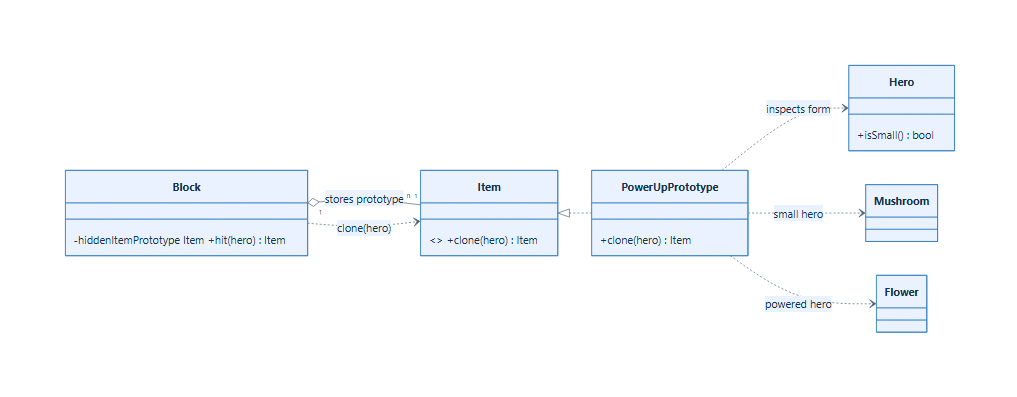
\includegraphics[width=0.88\textwidth,height=0.48\textheight,keepaspectratio]{img/diagrams/pattern-prototype.png}
\caption{Prototype supports repeated and context-sensitive hidden items.}
\end{figure}

\subsection{Facade Pattern}
\label{subsec:facade-pattern}

\texttt{LevelRuntime} is the facade for one live level.  \texttt{PlayingState}
does not directly coordinate every entity collection, collision pass, goal, or
map object.  It constructs the facade, calls \texttt{update}, calls
\texttt{renderWorld}, queries the hero and active region, and reacts to the
returned \texttt{LevelUpdateResult}.

Behind that interface, \texttt{LevelRuntime} owns \texttt{GameWorld},
\texttt{WorldPhysicsSystem}, and \texttt{InteractionSystem}; delegates initial
construction to \texttt{LevelBuilder}; caches playable regions and pipe routes;
maintains the active theme and fall boundary; enforces the boss-arena boundary;
performs cleanup; and exposes goal completion.  The facade makes the per-frame
ordering explicit while keeping scene presentation in \texttt{PlayingState}.

\subsection{Object Pool Pattern}
\label{subsec:object-pool-pattern}

\texttt{SoundManager} loads sound buffers once and keeps a bounded vector of
\texttt{sf::Sound} channels.  When an effect is requested, it first searches
for a stopped channel and reuses it; only when no stopped channel exists does it
allocate another channel, up to \texttt{m\_maxSfxChannels}.  This is a small
Object Pool that permits overlapping sound effects without allocating a new
SFML sound object for every event or allowing the number of active channels to
grow without limit.  Background music is handled separately as a streamed
\texttt{sf::Music} object.

\subsection{Pattern Collaboration and Design Consequences}
\label{subsec:pattern-collaboration}

The patterns are most valuable in combination.  The Singleton owns the screen
State context and long-lived audio service.  A selected screen constructs the
Level Facade.  The Facade delegates data-driven construction to Factories and
stores products in \texttt{GameWorld}.  During play, Hero and Enemy State
objects select short-term behavior, while the Hero Form Strategy selects the
orthogonal power policy.  Prototype creates context-sensitive block rewards,
and Observer-style callbacks publish spawned objects and sound events without
transferring control of the complete world to an entity.

The implementation consistently uses RAII ownership to reinforce these
patterns.  Screens, entities, forms, states, and projectiles are normally held
by \texttt{std::unique\_ptr}; the HUD is a \texttt{std::shared\_ptr} because it
must survive transitions and retries; service links and callback captures are
non-owning.  This makes destruction deterministic and documents whether a
relationship means ownership, sharing, or temporary collaboration.
\par
\endgroup
